\newpage
\section{Implementation, Testing, and Maintenance}

Pilot implementation of the project has been done with many features and interactive interface. Then we have done Testing by adding the users, uploading the transcripts of the particular user and then viewing the transcripts after login. 
\subsection{Introduction to Languages, IDE’s, Tools and Technologies used for
Implementation}
\begin{itemize}
    \item Python Language: Python is a widely used general-purpose, high level programming language. It was designed with an emphasis on code readability, and its syntax allows programmers to express their concepts in fewer lines of code. Python is a programming language that lets you work quickly and integrate systems more efficiently.
    \item IPFS: Interplanetary File System is a peer-to-peer protocol where each node stores a collection of hashed files. A client who wants to retrieve any of those files enjoys access to a nice abstraction layer where it simply needs to call the hash of the file it wants. IPFS then combs through the nodes and supplies the client with the file. It is a decentralized way of storing and referring to files but gives you more control and refers to files by hashes, allowing for much richer programmatic interactions.
    \item Flask: Flask is a web framework. This means flask provides you with tools, libraries and technologies that allow you to build a web application. This web application can be some web pages, a blog, a wiki or go as big as a web-based calendar application or a commercial website.
    \item HTML: HTML stands for Hyper Text Markup Language. It is the standard markup language for creating Web pages. It describes the structure of a Web page. It consists of a series of elements. HTML elements tell the browser how to display the content.
    \item SASS: Sass stands for Syntactically Awesome Stylesheet. It is an extension to CSS. It is a CSS pre-processor. It is completely compatible with all versions of CSS. It reduces repetition of CSS and therefore saves time.
    \item Javascript: JavaScript is a lightweight, cross-platform, and interpreted compiled programming language which is also known as the scripting language for webpages. It is well-known for the development of web pages, many non-browser environments also use it.
\end{itemize}
\subsection{Coding standards of Language used }
\begin{itemize}
    \item Writing Well-Structured Code
    \item Having Proper Comments
    \item Proper Naming of Variables, Classes, Functions and Modules
    \item Writing Modular Code
    \item Exception Handling for every critical situation
    \item Use the ‘with’ statement while opening a file, the ‘with’ statement closes the file even if there is an exception raised
\end{itemize}

\subsection{Project Scheduling using various tools such as PERT, GANTT charts, Open PROJ etc.}

\begin{figure}[h]
    \centering
    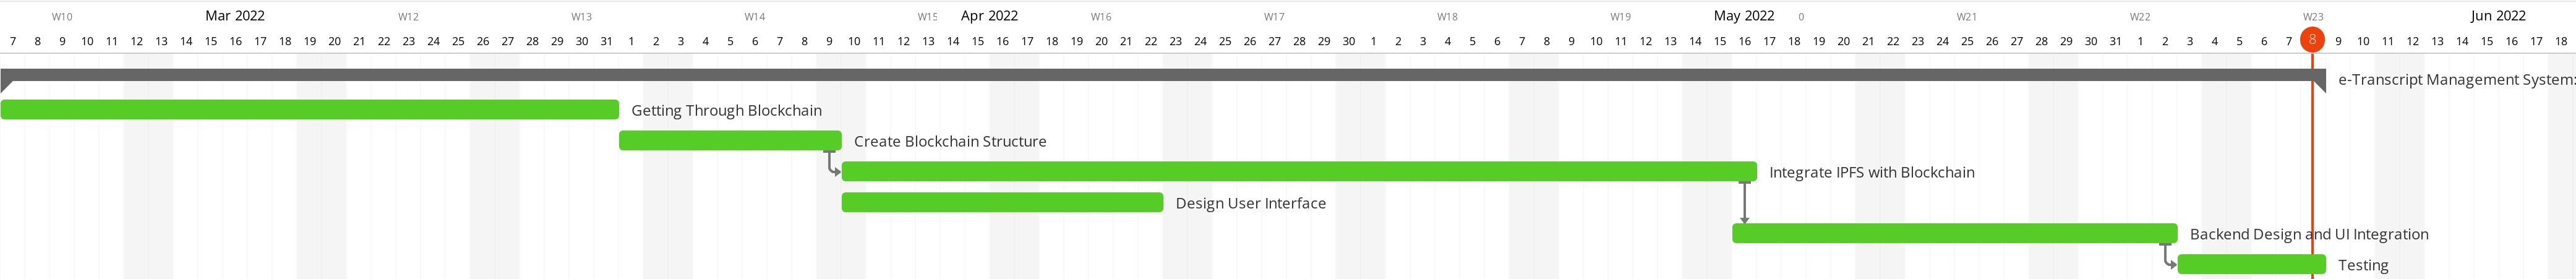
\includegraphics[scale=0.16]{images/gantt chart.jpg}\\[0.5cm]
    \caption{Gantt Chart}
    \label{fig:Gantt Chart}
\end{figure}
\begin{figure}[h]
    \centering
    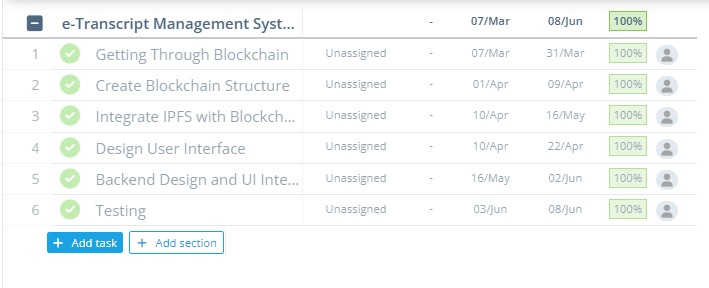
\includegraphics[scale=0.60]{images/gantt chart descriptions.jpeg}\\[0.5cm]
    % \caption{Gantt Chart Description}
\end{figure}
\newpage


\subsection{Testing Techniques and Test Plans}
We have prepared these testing techniques and test plans:
\begin{itemize}
    
    \item \textbf{Functional Testing:} Functional Testing plays an important role in Blockchain Testing as it helps in evaluating business requirements, processes, and effectiveness of use cases. Below are the components that can be tested as part of functional Testing:
    \begin{enumerate}
        \item Blockchain has been tested by adding blocks and then also verifying whether our blockchain is valid or not. 
        \item Also it has been tested that if we chain data of one block then whether it will affect the hash of that block or not.
        \item If we will add a block, it will add to the next of last block or not. 
        \item Whether Each student can access his/her certificates or not from our website.
    \end{enumerate}
    \item \textbf{Integration Testing:} Blockchain application work in multiple environments. So, it is important to test inter-system connections. We have tested whether our project working fine after integrating every components or not. Whether it is encrypting the file while uploading on IPFS, after it got integrated with whole project.
    
    \item \textbf{Performance Testing: } It helps in identifying hardware and software bottlenecks in advance. It helps to figure out the potential costs of running the application in the cloud or other environments.
    \item \textbf{Node Testing: }All diverse nodes on the Network has been tested independently to ensure smooth cooperation. 
    \item \textbf{API testing: } Application Programming Interface tests the interaction between applications in the blockchain ecosystem. API Testing ensures that requests and responses are formatted and operated properly. For this, we have tested whether our data that we are collecting from  , whether they are submitted in the database or not using post request and dashboard is able to get the data when it will be opened or not.
\end{itemize}



